\section{Theoretische Grundlage und Schematischer Aufbau des Versuches}
\label{sec:Theorie}
Ziel des Versuches ist es den glühelektrischen Effekt genauer zu untersuchen. Dafür soll die Austrittsarbeit von Wolfram bestimmt und deren Temperaturabhängigkeit nachvollzogen werden. \\
Um eine Wechselwirkung der freien Elektronen mit den Gasmolekülen zu verhindern wird das Experiment im Hochvakuum durchgeführt. Der schematische Aufbau ist in Abbildung \ref{fig:SHD} zu sehen.

\begin{figure}
  \centering
  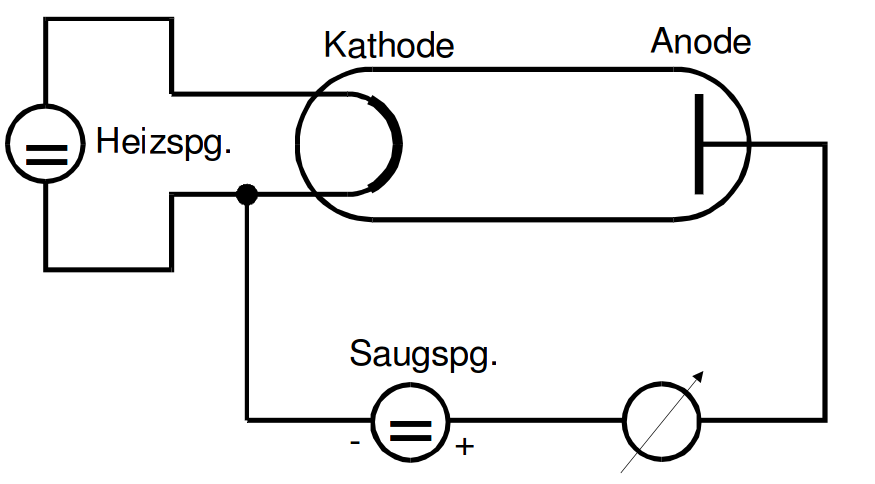
\includegraphics[height=5cm]{picture/Diode.png}
  \caption{Schaltung einer Hochvakuum-Diode \cite{pra}}
  \label{fig:SHD}
\end{figure}

Die Kathode wird durch einen Heizstrom $I_\text{H}$ erhitzt und die dadurch freigesetzten Elektronen mittels einer Beschleunigungsspannung $U_B$ in Richtung der Anode abgesaugt. Der zwischen den Anode und Katode fließende Strom $I_\text{S}$ wird in einem Diagramm gegen die Beschleunigungsspannung aufgetragen (siehe Abbildung \ref{fig:Ken}), und die Kennlinie in drei Gebiete eingeteilt.
\begin{figure}
  \centering
  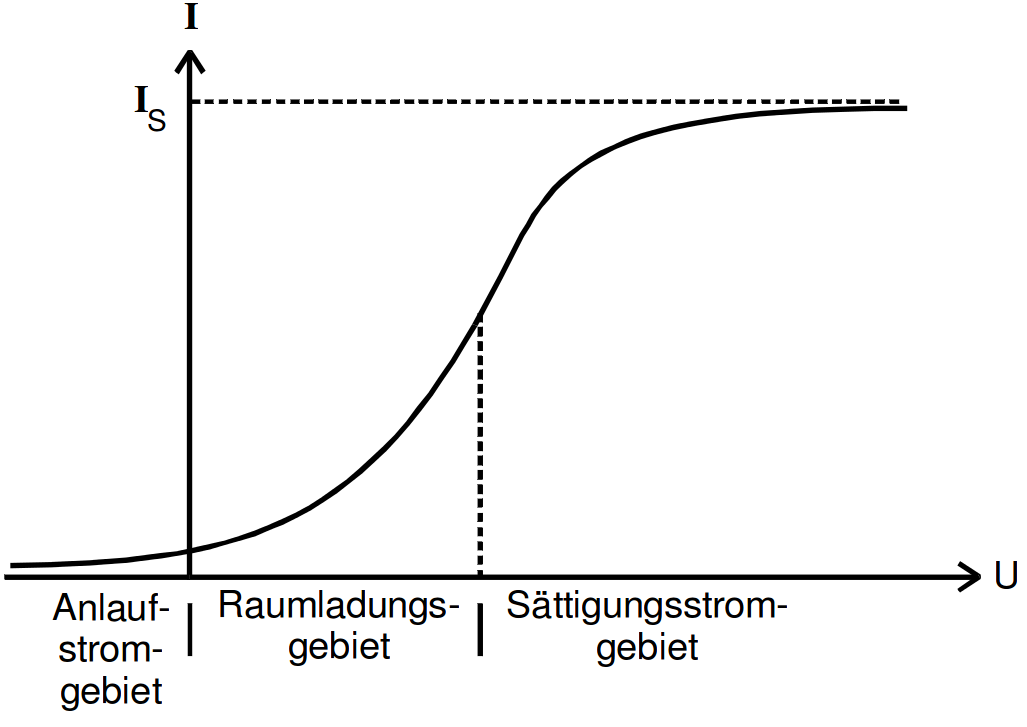
\includegraphics[height=5cm]{picture/Kennlinie.png}
  \caption{Kennlinie einer Hochvakuum-Diode. \cite{pra}}
  \label{fig:Ken}
\end{figure}
Das Gebiet, wo eine kleine Gegenspannung angelegt wird, wird als Anlaufstromgebiet bezeichnet. Der Strom $I_\text{S}$ ist darauf zurückzuführen, dass die aus der Kathode austretenden Elektronen eine statistisch verteilte Bewegungsenergie besitzen die ausreicht, die Gegenspannung zur Anode zu überwinden. Die Stromdichte berechnet sich in Abhängigkeit der Temperatur nach:
\begin{equation}
  j(V) = j_0 \exp\left( - \frac{e_0 V}{k_\text{B} T} \right)
  \label{eqn:jv}
\end{equation}
Anschließend an das Anlaufstromsgebiet befindet sich das Raumladungsgebiet. Es ist dadurch gekennzeichnet, dass nicht alle Elektronen von dem Feld abgezogen werden und einige der Feldlinien bereits vor der Kathode enden. Dies geschieht, da die Raumladungsdichte aufgrund der Bewegung der Elektronen abnimmt.
\begin{equation}
  j = \rho\, v
  \label{eqn:j}
\end{equation}
Daher muss das ohmsche Gesetz in diesem Bereich durch das Langmuir-Schottkysche Raumladungsgesetz
\begin{equation}
  j = \frac{4}{9}\, \varepsilon_0\, \sqrt{2\, e_0/m_0}\frac{V^{\frac{3}{2}}}{a^2}
  \label{eqn:jLS}
\end{equation}
ersetzt werden. Ziel des Versuches ist es die Beziehung $j \propto V^{3/2}$ zu bestätigen.
An das Raumladungsgebiet schließt sich das Sättigungsgebiet an. Dabei erreichen alle  Elektronen, die die Katode verlassen, die Anode. Der Sättigungsstrom sollte nun durch die Richardson-Gleichung beschrieben werden und noch von der Austrittsarbeit sowie der Temperatur abhängen.
\begin{equation}
  j_\text{s} (T) = 4\, \pi\, \frac{e_0\, m_0\, k_\text{b}^2}{h^3}\, T^2\, \exp \left( \frac{-e_0\, \Phi}{k_\text{B}\, T} \right)
  \label{eqn:js}
\end{equation}

\subsection{Fehlerrechnung}
Sämtliche Fits werden Mithilfe der Funktion "lmfit" aus Python gefittet und die Parameter ausgegeben.
